\section{Gameplay Block Design}
\label{sec:game}

The gameplay module will model the physics of the game, as well as output video information to be displayed on screen. Based on information from the grab button, player hand position, and hcount and vcount signals, it will see which of the player's hands are grabbing holds, and simulate their movement accordingly. The hcount and vcount signals indicate which pixel on screen is currently being evaluated, and will be the same as used in the tracking module. It will then send this information to the VGA out component of the labkit. Additionally, a feedback signal will be sent to the glove module to signal when a player is grabbing. 

The gameplay module will be broken up into four submodules: hand-holds, grabbing, movement, and pixel information.  The hand-holds module will keep track of where the hand holds are on the game map, and which onscreen pixels are occupied by hand holds. The grabbing module will take information from the hand holds, player hand positions, and grab button, to decide whether the player is grabbing onto any of the holds. If he is, the corresponding glove will be sent a haptic feedback signal.  This information will also be sent to a movement module. The movement module will use the players hand positions, and whether each hand is grabbing onto a hold to simulate movement of the player. Finally, the pixel information module will take the pixel by pixel information from the hand holds, as well as of the positions of the players hands, to output pixel by pixel information, as well as its corresponding hcount and vcount signals, to the VGA out component of the labkit.

\begin{figure}[h]
\centering
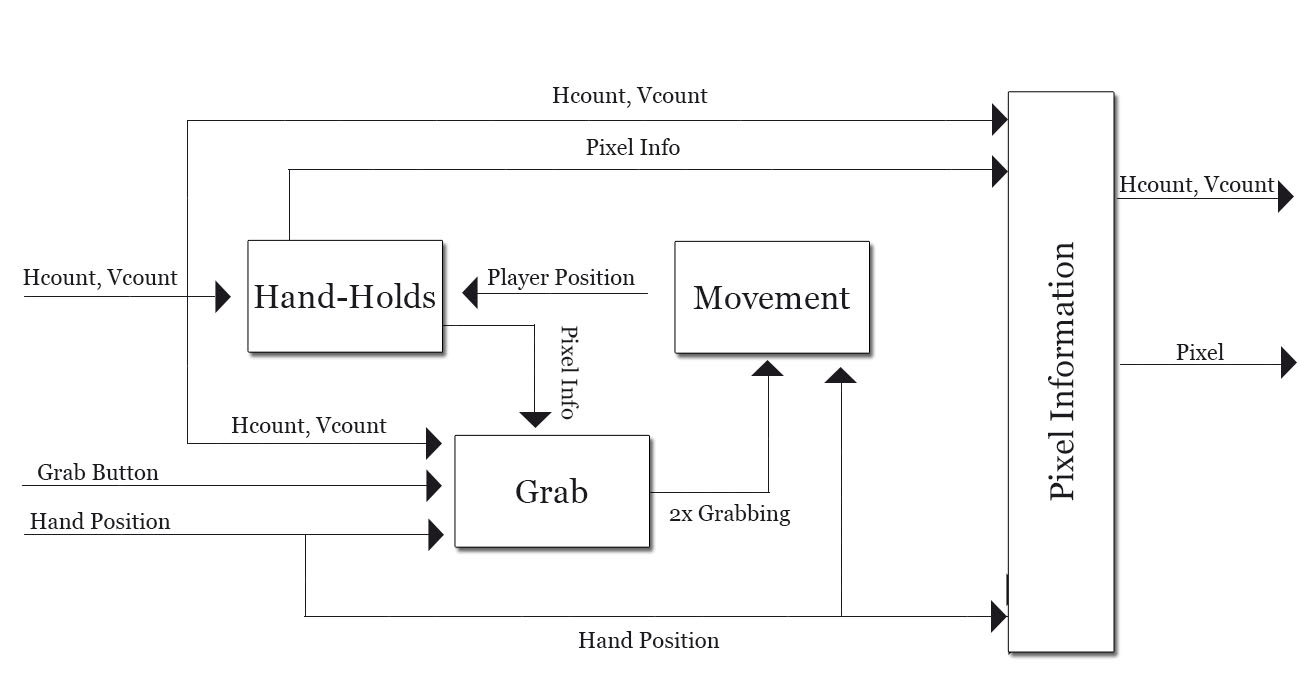
\includegraphics[width=6.5in]{img/gameplay.png}
\caption{The gameplay block is comprised of four modules: hand-holds, grabbing, movement, and pixel information}
\label{fig:gameplay block}
\end{figure}

The internal game map will be large, and only a portion of it, centered around the position of the player, will be shown on the screen. Because of this, there will be a mixing of relative and absolute positions during calculations. The absolute positions are in relation to the map as a whole, and relative positions are in relation to what is shown on the screen. 

\subsection{Hand-Holds}

The hand-hold submodule will in fact be multiple submodules, however they will act as one. Each instance of the hand-hold module will represent a single hold in the map, and will have an x and y coordinate associated with it, indicating its absolute position. The holds will also have a width and a length, over which the holds are present. 

Each hold sub-module will take in an hcount and vcount signal, as well as the screen's absolute position information and determine, pixel by pixel, whether a hand hold is present. This will be done by adding the screen x and y coordinates to the hcount and vcount coordinates, and seeing if they lie within the width and height of each modules x and y coordinates. If it does, it will output a “one”, associated with the corresponding hcount and vcount signal. If not it will output a “zero”. The outputs of all of the individual hand hold modules with then be anded together to signal if the current pixel, indicated by hcount and vcount, is occupied by any hand hold. 

Initially, the placement of the hand holds will be predetermined. However, if time permits, a map editor module will also be implemented. By flipping a switch, the player can enter this editing state. While in this state, the virtual camera position will be controlled by onboard buttons, and a cursor will be controlled by the right hand position. Clicking the right hand grab button will create a hand hold, and clicking a left hand button will delete one. This is a lofty goal, and the details are not yet worked out, but could be implemented if there is time. 

\subsection{Grabbing}

For each hand, a grabbing module will determine whether or not the player is currently grabbing onto a hand hold, updating its output at every vsync. It will do it in a similar, pixel by pixel, manner as done in the hand-hold module. Its inputs will be hcount and vcount signals, the pixel by pixel information coming from the holds, hand positions relative to the screen, and signals coming from both of the grab buttons. It will have one output registers, “grab”, for each of the two hands. When hcount and vcount are equal to one of the relative hand positions, it will check to see if the player is pressing the corresponding grab button and if there is a hand hold at that pixel. If these are all true, then it will signal to make the next output a one. Otherwise it will be made a zero. Additionally, this will be send to the glove to signal haptic feedback, as well as to the movement module.	

\subsection{Movement}

The movement module will be in charge of determining the players absolute position. It will use the player's relative hand positions, which of his hands are grabbing holds, and his previous velocity to do so. In actuality, the players position will always be fixed in relation to the camera, and will always be displayed as a fixed-position circle onscreen, so the movement module will actually be updating the screen position. The screen position is then fed back to the hand-hold modules at every vsync. 

The movement module will have two different states: one for when the player is currently grabbing a hold, and one for free-fall. If the player is grabbing a hold, their position will be determined by an “anchoring” hand. This is to avoid complications due to the player grabbing holds with both hands, and moving them in a way that violates the game. Typically, the anchoring hand will be the hand that the player most recently grabbed a hold with. However, if the player lets go with the anchoring hand, the movement module will assign the other as the anchoring hand. Whenever a hand becomes the anchoring hand, its current relative position will be stored, as will the absolute position of the screen. 

When a player is grabbing a hand hold, the movement module will update the camera position based on how far the anchoring hand has moved since it first anchored. It will subtract the current relative hand position from its relative anchored position and add it to the stored absolute screen position. If a player moves his anchored hand down, the screen will also shift down, allowing the player to reach a higher hand-hold with his non-anchored hand.

If the player is not grabbing any hand-hold, he will be in freefall, with a corresponding x and y velocity. When he first releases his hand, the gameplay module will take an average of his most recent velocities in the x and y directions, and set that to his freefall velocity. With each frame, the movement module will update the camera position based on this velocity, and the y velocity will be decremented in order to simulate gravity. This will allow the player to quickly pull down and release his grip, propelling him high into the air in order to grab a previously unreachable hold. 


\subsection{Pixel Information}

The pixel information module will output a color, along with appropriately pipelined hcount, vcount, and vsync information to a VGA output. It will take hcount and vcount signals, pixel information from the hand-hold module, and player hand position to determine the value of the current pixel output. It will first check to see if the hcount and vcount signals are within a small radius from the hand positions. If so, it will set the pixel output to red, signifying player hand position. Otherwise it will check to see if the hcount and vcount signals are within a small radius from the center of the screen. If so it will set the pixel output to green, signifying the players position. Otherwise, it check to see if the pixel information from the hand-hold module is true. If so, it will set the pixel output to yellow, otherwise black.  

\subsection{Game Module Complexity}

The game module is a relatively simple design. It does not rely on a large number of multipliers or memory, and all buses between modules are at most 16 bits wide. The grab, movement, and pixel information modules each use less than ten multiplexers, adders, and multipliers. The largest submodule is most likely the hand hold module. The hand-hold module will be created by many smaller modules, each representing a single hold on the map. Each of these will be comprised of  four 16 bit adders, and four 16 bit logic gates. If there are 25 hand holds on the map, this will amount to 100 16 bits adders and logic gates, which is still within the capacity of the labkit.

\subsection{Module Timeline and Testing}

There are four gameplay sub-modules that must be completed and integrated by the project deadline December 9, all of which will be done by Chris Lang. The hand-hold module has already been written. By November 12, the pixel calculator and grabbing modules should be completed. By November 14, the movement module should be completed. The week of the 18th can then be devoted to integrating the entire gameplay module. The week of the 25th is thanksgiving, and will be used to tie up loose ends within the gameplay module, and begin to integrate with the tracking module. The final week of December 2nd will then be used to finalize the project, finish integrating the major modules, and attempt to incorporate stretch goals if time permits.

Each sub-module will have to be tested individually. During testing, onboard buttons will be used to simulate hand position. The pixel calculator will be the first to be tested. Testing will ensure that the hand positions, as well as the player position, are correctly being displayed on screen, and that overall video output works. Then the hand-hold module can be tested. The screen position will stay fixed, and a few hand-holds will be placed on the game map. If the hand-hold modules work correctly, they will be displayed on screen along with the hand and player positions. Next, the grabbing module will be tested by using the the onboard buttons to simulate the hand positions and the grab buttons. If the grab module detects that a hand is currently grabbing, it will light up an led, signifying that it is working correctly. Finally, the movement module will be tested by using the onboard buttons to grab a hold, and move the player position. If this works, then the entire gameplay module is functioning correctly, and it is ready to be integrated with the tracking module. 

